\zotelo{../thesis.bib}
\def\bB{{\mathbf B}}
\def\bj{{\mathbf j}}
\def\bE{{\mathbf E}}
\def\rhoGJ{\rho_{\rm GJ}}
% \def\bOm{\mathbf{\Omega}}
\def\rpc{r_{\rm pc}}
\def\Apc{A_{\rm pc}}
\def\RLC{R_{\rm LC}}
\def\RNS{R_{\rm NS}}
\def\A{{\cal A}}
\def\B{{\cal B}}
\def\Ntrap{N_{\rm trap}}

\def\beq{\begin{equation}}
\def\eeq{\end{equation}}
\def\Eq{Equation}
\def\Eqs{Equations}
\def\Sect{Section}

\chapter{Polar-Cap Discharge}
\label{chap:polar-cap}

\section{Introduction}

Magnetic field lines that pass through the light cylinder of a rotating neutron
star are twisted and carry electric currents $\mathbf{j}_B=(c/4\pi)\nabla\times\bB$.
These currents are sustained by electric field $E_\parallel$ induced along
the magnetic field $\mathbf{B}$, and ohmic dissipation $E_\parallel j$ feeds the
observed pulsar activity. The value of $E_\parallel$ controls the
energies of accelerated particles, creation of secondary electron-positron
pairs, and emission of radio waves. The accelerating voltage has been discussed in
many works on pulsars beginning from early papers in the 1970s
% \citep{1971ApJ...164..529S, 1975ApJ...196...51R, 1969ApJ...157..869G}.
\citep{sturrock_model_1971, ruderman_theory_1975, goldreich_pulsar_1969}
% \cite{cheng_energetic_1986}
% \cite{goldreich_pulsar_1969}

The key dimensionless parameter of the polar-cap accelerator is
\begin{equation}
\label{eq:alpha}
   \alpha=\frac{j_B}{c\rho_\mathrm{GJ}},
\end{equation}
where $\rho_\mathrm{GJ}=-\bOm\cdot\mathbf{B}/2\pi c$ is the local corotation charge density of
the magnetosphere
% \citep{1969ApJ...157..869G}.
% (Goldreich \& Julian 1969).
\citep{goldreich_pulsar_1969}.

For a special value of $\alpha=\alpha_0$ (close to unity) a steady state was
found for the polar-cap flow with significant particle acceleration
% \citep{1977ApJ...217..227F, 1992MNRAS.255...61M}.
% (e.g. Arons \& Scharlemann 1979; Muslimov \& Tsygan 1992).
\citep{arons_pair_1979,muslimov_general_1992}.
However, $\alpha$ is not, in general, expected to take this special value
% \citep[e.g.][]{springerlink:10.1007/BF00172211}
% (e.g. Kennel et al. 1979).
\citep[e.g.][]{kennel_pulsar_1979}.
Global solutions for approximately force-free pulsar magnetospheres give
$\alpha$ that significantly varies across the polar cap
% \citep{MNR:MNR10192}.
% (Timokhin 2006).
\citep{timokhin_force-free_2006}.
In general, $\alpha$ can take any value from $-\infty$ to $+\infty$, depending
on the polar cap distance from the rotation axis and the location inside the
polar-cap region.

The character of the polar-cap accelerator strongly depends on $\alpha$
% \citep[hereafter B08]{1985MNRAS.217..443M, 2008ApJ...683L..41B}
% (Mestel et al. 1985; Beloborodov 2008, hereafter B08).
\citep[hereafter B08]{mestel_axisymmetric_1985, beloborodov_polar-cap_2008}
The solution with $\alpha=\alpha_0\approx 1$ is a separatrix between two
opposite regimes of efficient and inefficient acceleration.\footnote{
      Hereafter we will refer to this separatrix as $\alpha=1$, neglecting the
      deviation of $\alpha_0$ from unity. Precise $\alpha_0$ depends on
      the curvature of magnetic field lines and the general
      relativistic effects
      % \citep{1992MNRAS.255...61M}
      % (Muslimov \& Tsygan 1992);
      \citep{muslimov_general_1992};
      its exact value is close to unity and
      is not essential for the rest of the paper.}
In particular,  if $0<\alpha<1$, $E_\parallel$ is quickly screened in the
charge-separated plasma flowing from the polar-cap surface. The electric field
satisfies
Maxwell equations that read
\citep[in the co-rotating frame of the star, see e.g.][]{fawley_potential_1977,levinson_large-amplitude_2005}
  % (in the co-rotating frame of the star, see e.g. Fawley et al. 1977; Levinson et al. 2005),
\begin{equation}
\label{eq:Gauss}
   \nabla\cdot\bE=4\pi(\rho-\rho_\mathrm{GJ}),
 \end{equation}
 \begin{equation}
 \label{eq:Maxw}
   \frac{\partial\bE}{\partial t}=4\pi(\mathbf{j}_B-\mathbf{j}).
\end{equation}
If $0<\alpha<1$, there exists a velocity $v=\alpha c$ that allows the charge-separated
flow $j=\rho v$ to satisfy both conditions $\rho=\rho_\mathrm{GJ}$ and $j=j_B$.
If the flow started from the conducting boundary (which has $E=0$) with
$v=\alpha c$, no electric field would be generated (then $\nabla\cdot\bE=0$
and $\partial\bE/\partial t=0$). The actual boundary has $v\neq \alpha c$, as
charges are lifted from the polar-cap surface with a small initial $v$,
comparable to the thermal velocity in the surface material.
The deviation of $v$ from $\alpha c$ implies $\rho\neq\rho_\mathrm{GJ}$ or
$j\neq j_B$, which generates electric field.
B08 argued that
equations~(\ref{eq:Gauss}) and (\ref{eq:Maxw}) with $0<\alpha<1$
always drive the flow toward $v=\alpha c$,
like a pendulum is driven by gravity toward its equilibrium position.
The resulting oscillations occur in space or time,
according to equations~(\ref{eq:Gauss}) or (\ref{eq:Maxw}), respectively.
For example, the steady-state solution for a cold flow exhibits
oscillations in space
% \citep[B08]{1985MNRAS.217..443M}
\citep[B08]{mestel_axisymmetric_1985}
   % (Mestel et al. 1985; B08).
The oscillatory behavior of the flow with $0<\alpha<1$ is, in essence, Langmuir
oscillations; they are generated near the boundary where the flow is initially
accelerated toward $v=\alpha c$.

In this chapter, we investigate the accelerator with $0<\alpha<1$ in more
detail. In \Sect~\ref{sec:pc-steady-state}, we write down the steady-state
solution for the charge-separated flow, generalized to non-zero temperature of
the polar-cap. We argue that the flow is unstable to small perturbations and can
develop into a complicated time-dependent state with a broad momentum
distribution. To explore the behavior of the flow, we perform fully kinetic
time-dependent simulations. The method of simulations is described in
\Sect~\ref{sec:pc-setup}, and the results are presented in
\Sect~\ref{sec:pc-results}. In \Sect~\ref{sec:pc-ions} we consider the flow with
mixed species of ions extracted from the surface. Our simulations show the
turbulent oscillatory behavior of the flow with $0<\alpha<1$; particle
acceleration in the flow is insufficient to ignite pair creation. Implications
of this ``dead zone'' for radio emission and outer gaps in pulsars are discussed
in \Sect~\ref{sec:pc-discussion}.


\section{Steady-state solution for a charge-separated flow}
\label{sec:pc-steady-state}


\subsection{Basic equations}


It is natural first to attempt to construct a simplest model
assuming that the polar-cap flow is steady in the (rotating) frame of the neutron star.
Given the steady magnetic field in this frame,
and the steady boundary conditions at the stellar surface --- excellent
static conductor that can supply charges with a given temperature, --- one
could expect a steady state to be established unless the flow is prone to an instability.

Consider a charge-separated flow from the polar cap that carries electric current
$j_B$ along magnetic field $\mathbf{B}$ (because of a strong field, particles are kept in
the ground Landau state).
In a steady state $j=j_B$ (equation~\ref{eq:Maxw}).
For simplicity, let us assume that $\mathbf{B}$ is approximately perpendicular to
the polar cap and let $z$ measure the altitude above the stellar surface.
A particle of mass $m$ and charge $e$ that starts with a Lorentz factor
$\gamma_0\approx 1$ at $z=0$ will accelerate as it moves along the magnetic
field line,
\begin{equation}
\label{eq:a}
    \gamma(z)=\gamma_0+a(z),  \qquad a=-\frac{e(\Phi-\Phi_0)}{mc^2},
\end{equation}
where $\Phi$ is the electric potential.
Gravitational acceleration (and centrifugal acceleration in the rotating frame) is
neglected compared to the electric acceleration.

The electric potential satisfies Poisson equation,
\begin{equation}
\label{eq:Phi}
    \frac{d^2\Phi}{dz^2}=-4\pi(\rho-\rho_\mathrm{GJ}),
\end{equation}
where we assumed that the potential varies along $z$ much faster than in
the transverse directions, i.e. the acceleration length $l_\parallel$ is much smaller
than the characteristic transverse scale of the problem $l_\perp$, which may be
associated with the size of the polar cap. This condition is satisfied for the flows considered below.\footnote{
      Alternatively, the additional term $\nabla_\perp^2\Phi$ could be moved to the
      right-hand side of equation~(\ref{eq:Phi}) and included in the effective $\rho_\mathrm{GJ}$.}
The term $-\rho_\mathrm{GJ}$ may be viewed as a fixed background charge density.
The charge density of the flow itself is given by
\begin{equation}
     \rho(z)=j_B \int_1^{\infty} \frac{w(\gamma_0)\,d\gamma_0}{v(\gamma_0,z)}.
\end{equation}
Here $v(\gamma_0,z)$ is the velocity of particles that started at $z=0$
with initial Lorentz factor $\gamma_0$; note that $v^2/c^2=1-\gamma^{-2}$ where
$\gamma(z)$ is given by equation~(\ref{eq:a}).
Function $w(\gamma_0)$ describes the probability distribution of $\gamma_0$.
The width of this distribution is controlled by the temperature of polar cap $T$.
For example, $w=\delta(\gamma_0-1)$ describes a cold polar cap ($T=0$) where
all particles have $\gamma_0=1$.

We multiply both sides of equation~(\ref{eq:Phi}) by $da/dz=-(e/mc^2)d\Phi/dz$ and find,
\begin{equation}
\label{eq:diff}
     \frac{mc^2}{2e}\,\frac{d}{dz}\left(\frac{da}{dz}\right)^2
   =4\pi\left[
   \frac{j_B}{c}\int_1^{\infty} \frac{dp}{dz}(\gamma_0,z)\,w(\gamma_0)\,d\gamma_0
         -\frac{da}{dz}\,\rho_\mathrm{GJ}\right].
\end{equation}
On the right-hand side, we used $da/dz=-d\gamma/dz$ (equation~\ref{eq:a}) and
$d\gamma/v=dp/c$. Integration of equation~(\ref{eq:diff}) in $z$ gives
\begin{equation}
\label{eq:steady}
    \frac{\lambda_p^2}{2}\left(\frac{da}{dz}\right)^2
         \int_1^{\infty} \left[p(\gamma_0,z)-p_0\right]\,w(\gamma_0)\,d\gamma_0
           -\frac{a(z)}{\alpha},
\end{equation}
where
\begin{equation}
   p^2(\gamma_0,z)=\gamma^2-1=\left[\gamma_0+a(z)\right]^2-1.
\end{equation}
In equation~(\ref{eq:steady}) we used $a(0)=0$ and the boundary condition $da/dz(0)=0$
(the stellar surface is modeled as a perfect conductor that can freely emit charges
with $E_\parallel(0)=0$). We also used $j_B(z)\approx const$ and
$\rho_\mathrm{GJ}(z)\approx const$, as $j_B$ and $\rho_\mathrm{GJ}$ do not vary much on the
characteristic acceleration length $\lambda_p$, which is defined by
\begin{equation}
\label{eq:lambda}
   \lambda_p^2=\frac{mc^3}{4\pi e j_B}.
\end{equation}
This length may be thought of as the plasma skin depth; it is related to the
plasma frequency $\omega_p$,
\begin{equation}
   \lambda_p=\frac{c}{\omega_p}, \qquad \omega_p^2=\frac{4\pi n e^2}{m},
\end{equation}
with the characteristic plasma density $n=j_B/ec$.

A quick estimate for $j_B$ and $\lambda_p$ in pulsars may be obtained from
the following consideration. The magnetic flux through the polar cap $\Psi$ equals
the flux through the light cylinder $\RLC=c/\Omega$.
The bundle of open field lines is strongly twisted at the light cylinder
(toroidal component comparable to poloidal), and hence it carries
electric current $I\sim c\Psi/2\pi\RLC$, according to Stokes theorem.
The current density near the star satisfies $j_B/B\approx I/\Psi$
(which follows from the fact that $\mathbf{j}$ flows along $\mathbf{B}$), which yields
\begin{equation}
\label{eq:j_B}
     j_B\sim \frac{\Omega B}{2\pi}.
\end{equation}
This gives the plasma skin depth in the polar-cap accelerator,
\begin{equation}
    \lambda_p \sim \frac{c}{(\Omega\omega_B)^{1/2}},
    \qquad \omega_B=\frac{eB}{mc}.
\end{equation}
The scale $\lambda_p$ is much smaller than the typical size of the polar cap
$\rpc\sim(\RNS^3\Omega/c)^{1/2}$, where $\RNS\sim 10^6$~cm is the radius of
the neutron star.

%%%%%%%%%%%%%%%%%%
\begin{figure}[h]
%\epsscale{0.25}
  % \epsscale{1.0}
\begin{center}
  % \plotone{f1.eps}
  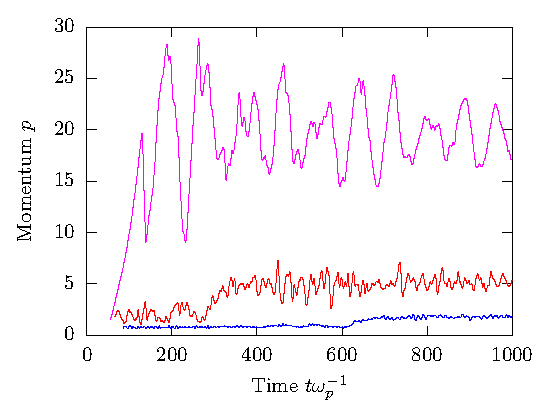
\includegraphics[width=0.7\textwidth]{pics/chap2/f1.eps}
  \caption[Steady-state solution for $\alpha < 0$]{Steady-state solution for the
    charge-separated polar-cap flow with $\alpha=0.8$. Two cases are shown: cold
    polar cap $T=0$ (solid curve) and warm polar cap $kT/mc^2=0.03$ (dashed
    curve), which corresponds to average injection momentum $0.22mc$. Dotted
    curve shows the solution for a cold flow where all particles are injected
    with the same $p_0=0.22$. }
\label{fig:steady}
\end{center}
\end{figure}
%%%%%%%%%%%%%%%%%%


\subsection{Cold and warm solutions}\label{sec:solutions}

Once the injection distribution $w(\gamma_0)$ is specified,
it is straightforward to numerically integrate equation~\eqref{eq:steady} and find $a(z)$.
In our sample models we chose
$w(\gamma_0)=(kT)^{-1}\exp[-(\gamma_0-1)/kT]$ with $kT/mc^2=0$ (cold) and
0.03 (warm); the average injection momentum $p_0$ in the warm model equals
$0.22mc$. Figure~\ref{fig:steady} shows $\Phi(z)$ for the cold and warm solutions.

Figure~\ref{fig:steady} also shows a third model where all particles injected at the polar cap
have $p_0=0.22$, i.e. $w(\gamma_0)$ is a delta-function.
In this model, equation~(\ref{eq:steady}) simplifies to
\begin{equation}
\label{eq:cold}
    \frac{\lambda_p^2}{2}\left(\frac{da}{dz}\right)^2 = p(\gamma_0,z)-p_0
                                                                               + \frac{a(z)}{\alpha},
\end{equation}
[same as equation~(3) in B08]. This flow is cold everywhere, i.e. its momentum
distribution is described by $f(p^\prime)=n\,\delta[p^\prime-p(z)]$.
As one can see in Figure~\ref{fig:steady}, the cold model with $p_0\neq 0$ provides an
excellent approximation to the exact warm model that has the same {\it average}
value of $p_0$.

The cold flow solution was discussed in earlier works
% \citep[B08]{1985MNRAS.217..443M}
\citep[B08]{mestel_axisymmetric_1985}
% (Mestel et al. 1985; B08).
For $1-\alpha\ll 1$, the oscillation period is approximately given by (B08)
\begin{equation}
    z_0 \approx 2^{3/2}\frac{\lambda_p}{1-\alpha}, \qquad 1-\alpha\ll 1.
\end{equation}
The precise period is obtained by numerical integration; e.g.
$z_0=11.0\,\lambda_p$ for $\alpha=0.8$.
The momentum of the steady cold flow $p(z)$ oscillates between the injection
momentum $p_0\ll 1$ and a maximum value $p_{\max}$. The minima and
maxima are where $da/dz=0$, and from equation~(\ref{eq:cold}) one finds
\begin{equation}
\label{eq:pmax}
    p_{\max}=\frac{2\alpha\,\gamma_0-(1+\alpha^2)p_0}{1-\alpha^2}.
\end{equation}


\subsection{Stability of the flow}


Although the cold solution with $p_0=0.22$ reproduces very well the electric
potential $\Phi(z)$ of the exact warm solution with the same average $p_0$,
the warm and cold flows are qualitatively different. Their different
momentum distribution functions $f(p,z)$ imply a qualitatively different response
to small perturbations.

Consider first the cold-flow solution
shown by the blue dotted curve in Figure~\ref{fig:steady}.
Since all particles are injected with the same momentum $p_0=0.22$,
all of them follow a single trajectory in the phase space $(z,p)$.
They periodically reach the minimum momentum equal to $p_0$ at
$z_k=kz_0$ ($k=0,1,...$) where potential $\Phi$ reaches maximum.
There are no particles with momenta $p\approx 0$, so
a small perturbation cannot force any particles to reverse their direction of motion,
and hence the perturbation will be advected along the flow.
This flow may be expected to be stable.

In contrast, the warm flow (dashed curve in Figure~\ref{fig:steady}) has a broad distribution
of $p_0$ that extends from $p_0=0$. At each peak of the electric potential
$z_k$ there is a population of particles with nearly zero velocities. Consider a
perturbation at $z\approx z_k$. For example, suppose
a small bunch $\A$ of particles with momenta in a range $(p_1,p_1+\Delta p)$
are slightly pushed forward while the rest of particles are unperturbed.
This perturbation implies a local increase in electric current $j>j_B$ and hence
$\partial E_\parallel/\partial t<0$ (equation~\ref{eq:Maxw}), generating negative
electric field $\delta E_\parallel$ at $z\approx z_k$ that tends to restore the
condition $j=j_B$. In contrast to the initial perturbation,
the induced $\delta E_\parallel$ affects {\it all} local particles, regardless their
momentum, not just bunch $\A$. This has two implications:
(1) The induced $E_\parallel<0$ will easily and quickly reduce $j$ back to $j_B$ but
will be unable to decelerate bunch $\A$ to the momentum it would have in the
steady state flow --- bunch $\A$ will continue to move to $z>z_k$ with a larger
momentum.
(2) $\delta E_\parallel<0$ will give very slow particles $p\approx 0$ negative velocities,
creating a new bunch $\B$ that slides backward down the potential hill. Bunch $\B$
creates $j<j_B$ at $z<z_k$, and the system reacts there by inducing a small
$\delta E_\parallel > 0$, which accelerates all local particles, regardless their momenta,
not just bunch $\B$. As a result, $j$ quickly recovers to $j_B$, however, bunch $\B$
is not stopped from moving backward and away from $z=z_k$.

Thus one can see that the perturbation creates a permanent damage
to the steady state that broadens the momentum distribution by creating backflowing
particles.
This perturbation is {\it not} advected away along the flow, and can develop further.
The backflowing particles turn out to be trapped between two peaks of the
electrostatic potential. Further development can be studied with kinetic time-dependent
simulations; it eventually completely destroys the steady state solution.


%#################################################################

\section{Numerical setup}
\label{sec:pc-setup}


Our numerical method is similar to that used by
% \citet[hereafter BT07]{2007ApJ...657..967B}
% Beloborodov \& Thompson (2007, hereafter BT07).
\citet[hereafter BT07]{beloborodov_corona_2007}
The plasma is modeled as a large number $N\sim 10^6$ of individual
particles that flow along the magnetic field lines.
We assume that the magnetic field is fixed in
the co-rotating frame of the star; thus $j_B$ and $\rho_\mathrm{GJ}$ are fixed. Then the
problem becomes essentially one-dimensional, as discussed in detail in BT07.
In the present chapter, we consider only charge-separated flows, with no pair creation.
Three other differences from the magnetar simulation in BT07 are as follows:
(1) The magnetar problem had $\alpha\gg 1$
($\rho_\mathrm{GJ}$ was negligible compared with $j_B/c$);
in contrast, $\rho_\mathrm{GJ}$ is crucial for polar-cap flows considered here.
(2) The presence of gravity was essential for the closed-field circuit considered
in BT07, where the global plasma flow was simulated (on a scale comparable to
the radius of the star); in the problem considered here the electric fields are
screened on a much smaller scale $\sim \lambda_p$ and the gravitational
acceleration plays no role.
(3) The flow behavior on the small scales $z\ll \RNS$ may be studied using
a smal computational box $H\ll \RNS$ with an open outer boundary (see below).

In the absence of pair creation, the flow is composed of particles lifted from
the surface; we assume that all of them have the same mass $m$ and charge $e$.
 The particle motion is described by the equation,
\begin{equation}
\label{eq:p}
    \frac{dp_i}{dt} = \frac{eE_\parallel(z_i)}{mc},   \qquad i=1,..,N,
\end{equation}
where $p_i$ is the momentum of the i-th particle in units of $mc$, and
$E_\parallel(z_i)$ is the self-consistent electric field at the particle location $z_i$.
The field is found by integrating Gauss law (equation~\ref{eq:Gauss})
along the magnetic field line,
\begin{equation}
 \label{eq:E}
   E_\parallel(z_i) = 4\pi \left[ eN(z_i) - \rho_\mathrm{GJ} z_i \right].
\end{equation}
Here $N(z_i)$ is the column density of particles between $z=0$ and $z=z_i$,
and we used the boundary condition $E_\parallel(0)=0$, as the material below the
stellar surface is assumed to be a very good conductor that can emit free charges.
Divergence of the perpendicular component of electric field $E_\perp$
is neglected in equation~(\ref{eq:E}) (see BT07 for discussion of this approximation).
The approximation $|\nabla_\perp\cdot\bE_\perp|\ll |dE_\parallel/dz|$ is valid if the
characteristic scale of the flow acceleration $z_0$ is smaller than the transverse
scale $l_\perp$, which is limited by the polar-cap size $\rpc$;
the condition $z_0\ll \rpc$ is satisfied in the dead-zone models presented below.
We also assume that $\rho_\mathrm{GJ}$ is approximately constant on scale $z_0$.
equations~(\ref{eq:p}) and (\ref{eq:E}) in essence describe a relativistic, time-dependent
diode problem with an additional fixed background charge density $-\rho_\mathrm{GJ}$.

As we track the motion of all particles individually, the continuity equation is
automatically satisfied; for a charge-separated flow it is equivalent to charge
conservation,
\begin{equation}
\label{eq:charge}
    \frac{\partial\rho}{\partial t}+\frac{\partial j}{\partial z}=0.
\end{equation}
equation~(\ref{eq:Maxw}) follows from equations~(\ref{eq:Gauss}) and (\ref{eq:charge}),
so we will not need equation~(\ref{eq:Maxw}).
Instead, the parameter $j_B$ enters the problem as a boundary condition.
The magnetic field lines are frozen in the excellent conductor below the stellar
surface, which sustains $j(0)=j_B$.
This condition is enforced in the simulation by injecting the charges in
the computational box at $z=0$ with the fixed rate $j_B$ (BT07).

The electric current $j_B$ is enforced at one boundary $z=0$. Since
the computational box has a finite size $H$, we also have to choose the
boundary condition at $z=H$ and the value of $H$. In all sample models
shown in this chapter we use the simplest boundary condition:
particles moving out of the box are lost and no particles enter the box at
$z=H$. This condition may be refined by allowing a small inflow of returning
particles at the outer boundary. We ran test simulations that show that the
refinements are not important as long as the boundary is sufficiently far,
so that $H$ is much greater than the characteristic scale of the flow acceleration.

In the one-dimensional model, the transverse
gradients are neglected, and the flow effectively has a slab geometry.
Then it is sufficient to follow particles flowing through a small area $A$ of the slab.
This allows one to chose a reasonable number of particles in the computational
box, $N\sim AHn$, e.g. $N\sim 10^6$, so that their dynamics can be followed
in a reasonable computer time. On the other hand,
$N$ should be large enough so that the plasma scale $\lambda_p$ contains
many particles $N_p=A\lambda_p n$.

In summary, we choose $N$ and $H$ so that
\begin{equation}
    \frac{H}{\lambda_p}\gg 1, \qquad N_p=\frac{\lambda_p}{H}\,N \gg 1.
\end{equation}
In this limit, the results are expected to be independent of the choice of $N$ and
$H$ (we verify this by varying the two parameters in Section~3.4). For most of our
simulations $H=100\lambda_p$ and $N\sim 10^6$. Another requirement is a small
time step of the simulation, $\Delta t\ll\omega_p^{-1}$, so that plasma oscillations
are well resolved.


%################################################################

\section{Results}
\label{sec:pc-results}

\subsection{Steady state tests}


In our simulations and in reality the plasma above pulsar polar caps is collisionless.
In the absence of pair creation it must satisfy
%  the collisionless Boltzmann
the Vlasov equation,
\begin{equation}
\label{eq:Vlasov}
    \frac{\partial F}{\partial t} + \mathbf{v}\cdot \nabla F + \frac{d\mathbf{p}}{dt}\cdot \nabla_\mathbf{p} F = 0,
\end{equation}
where $F(t,z,p)$ is the particle distribution function in phase space. The
electric current is $j(t,z)=\rho \bar{v}$ where $\bar{v}(t,z)$  is the average
velocity of the particles. As a first simple test, consider a uniform flow
with $\rho(z)=\rho_\mathrm{GJ}$, $\bar{v}(z)=\alpha c$, and $E_\parallel(z)=0$.
It is easy to see from equations~(\ref{eq:p}), (\ref{eq:E}) and (\ref{eq:Vlasov}) that
the flow must remain in this state. This behavior is reproduced by our simulations.
The steady uniform flow can have any momentum distribution $F(p)$
as long as $\bar{v}=\alpha c$. Note that it requires a continual injection of particles
at $z=0$ with the average velocity $\bar{v}=\alpha c$ (which also requires $0<\alpha<1$).

As a second test, consider a ``cold'' flow where all particles move with
momentum $p(z)$, with zero momentum dispersion. Suppose the flow is injected
at $z=0$ with velocity $v_0<\alpha c$. Then $E_\parallel$ must be generated,
accelerating the flow. In a steady state, the solution for the cold flow must have
the form, $F(z,p^\prime)=n(z)\,\delta[p^\prime-p(z)]$, where $p(z)$ and $n(z)$ can
be described analytically. We first test the special case $\alpha=1$
% \citep{1977ApJ...217..227F}.
% (Michel 1974).
\citep{michel_rotating_1974}.
The flow is accelerated by the self-consistent $E_\parallel(z)$, and $p$ exceeds
unity at $z\sim\lambda_p$. At heights $z\gg \lambda_p$, velocity approaches $c$,
charge density of the flow $\rho=j_B/v$ approaches $\rho_\mathrm{GJ}$, and
electric field $E_\parallel$ asymptotes to a constant value,
\begin{equation}
   E_\parallel=\left[\frac{8\pi m cj_B}{e}\left(\gamma_0-p_0\right)\right]^{1/2}
                      \left[1+{\cal O}(p^{-1})\right],
\end{equation}
where $\gamma_0=(1-v_0^2/c^2)^{-1/2}$ and $p_0=\gamma_0\beta_0$.
Then the flow momentum keeps growing linearly with $z$,
\begin{equation}
     p(z)=\left[2(\gamma_0-p_0)\right]^{1/2}\,\frac{z}{\lambda_p}, \qquad z\gg\lambda_p.
\end{equation}
This solution is reproduced by our simulations with ``cold injection'' --- all injected
particles at $z=0$ have velocity $v_0$. After an initial relaxation period
(comparable to the light crossing time of the computational box) the system
forgot initial conditions and relaxed to the steady state shown in Figure~\ref{fig:alpha1}
(in this example, $v_0=1/6$).
% (\citet{1977ApJ...217..227F}).
The charge density of the flow is large near the polar cap surface and asymptotes
to $\rho_\mathrm{GJ}$ at $z\gg\lambda_p$, as expected.

\bigskip

%%%%%%%%%%%%%%%%%%
\begin{figure}%[h]
% \epsscale{1}
%\epsscale{0.1}
\begin{center}
% \plottwo{f2a.eps}{f2b.eps}
   % \plotone{f2a.eps}\\
   % \plotone{f2b.eps}
  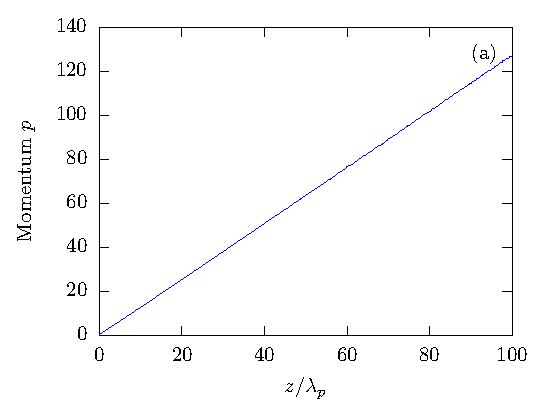
\includegraphics[width=0.6\textwidth]{pics/chap2/f2a.eps} \\
  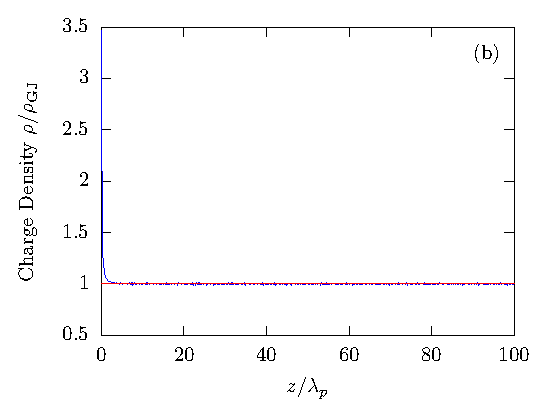
\includegraphics[width=0.6\textwidth]{pics/chap2/f2b.eps}
  \caption[Test run for a cold flow with $\alpha = 1$]{Test run for a cold-flow
    model with $\alpha=1$ and $v_0=c/6$. The flow relaxed to a steady state in
    the entire box $H=10^2\lambda_p$ on the light-crossing timescale, $H/c$; the
    state of the system is shown at $t = 10H/c$. (a) Flow momentum per particle
    $p(z)$ in units of $mc$. (b) Charge density $\rho(z)$.}
\label{fig:alpha1}
\end{center}
\end{figure}
%%%%%%%%%%%%%%%%%%

%%%%%%%%%%%%%%%%%%%
\begin{figure}%[h]
\begin{center}
%\epsscale{0.1}
% \epsscale{1.0}
%\plottwo{f2a.eps}{f2b.eps}\\
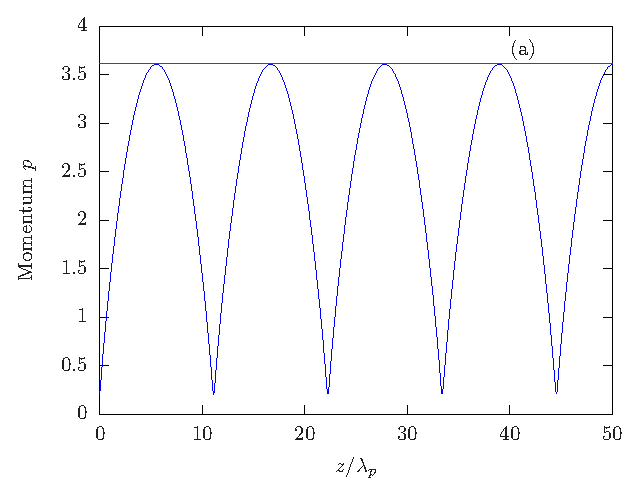
\includegraphics[width=0.6\textwidth]{pics/chap2/f3a.eps}\\
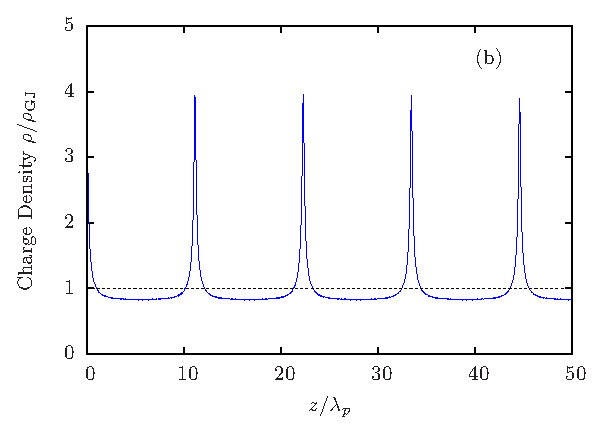
\includegraphics[width=0.6\textwidth]{pics/chap2/f3b.eps}\\
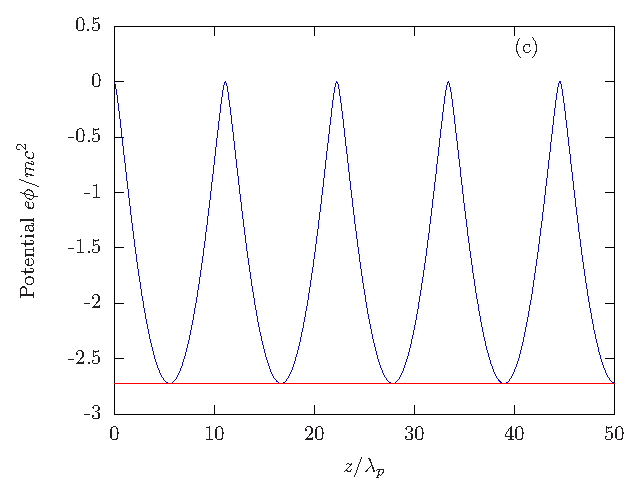
\includegraphics[width=0.6\textwidth]{pics/chap2/f3c.eps}
\caption[Snapshot of a cold flow with $\alpha < 0$]{Cold flow with $\alpha=0.8$ and $\beta_0=0.2$ at time $t=1.45H/c$
%  light-crossing time of the computational box.
% The box is divided into 500 bins and each plotted quantity
% is averaged over the bin.
(a) Momentum $p$ (in units of $mc$). (b) Charge density.
% The charge density peaks are so narrow that they are not fully resolved with
% 500 bins; their true full height is $\rho_{\max}=(\alpha/\beta_0)\rho_\mathrm{GJ}=4\rho_\mathrm{GJ}$.
(c) Electrostatic potential.
}
\label{fig:alpha0.8cold}
\end{center}
\end{figure}
%%%%%%%%%%%%%%%%%%%

Then we studied cold flows with $0<\alpha<1$ and fixed injection velocity $\beta_0$.
We chose in our sample numerical model $\alpha=0.8$ and $\beta_0=0.2$.
The computational box was initially empty; the plasma injected at $z=0$
filled the box on the dynamical timescale
$\sim H/c$ and established a steady state shown in Figure~\ref{fig:alpha0.8cold}.
The steady state is in perfect agreement with the analytical model of \Sect~2.2.
The charge density $\rho(z)$ has spikes at $z=kz_0$ ($k=0,1,...$) where
the flow has the minimum velocity $\beta_0$; the height of each spike is
$\rho_{\max}=j_B/\beta_0=(\alpha/\beta_0)\rho_\mathrm{GJ}$.
The charge spikes are associated with maxima of the electric potential (Figure~\ref{fig:alpha0.8cold}c).
The oscillating momentum has maxima $p_{\max}=3.6$, in excellent agreement
with equation~(\ref{eq:pmax}). The period of oscillation is $z_0\approx 11\lambda_p$, same
as found using the method of \Sect~2.2.

As anticipated in \Sect~2.3, we find that the steady state becomes unstable if we
reduce $\beta_0$ to zero. Then any small perturbation (e.g. due to numerical error)
completely destroys the steady state; instead, a time-dependent state forms, with a
broadened momentum distribution function.
A steady flow with a finite $\beta_0\neq 0$ can also be destroyed, although in this
case a finite,
sufficiently large perturbation is required. In fact, this case provides a better
setup for a numerical analysis of the instability,
as we can control the form of the initial perturbation and then observe how it destroys
the flow that was stable before the perturbation was applied.
We made such an experiment with the flow with $\alpha=0.8$ and $\beta_0=0.2$.
We applied a perturbation that was localized in space and time --- a small ``kick''
$\delta p$ was given to all particles located in a small region $\delta z=\lambda_p/2$;
in this experiment $\delta p$ had a Gaussian distribution with the mean value and
dispersion equal to 0.02.
We observed the following evolution. As the localized
perturbation moved along with the background flow, it was greatly amplified when it
reached the potential maximum (which corresponds to the minimum $p_0\approx 0.2$
of the steady-state solution,
see Figure~\ref{fig:alpha0.8cold}), and some particles acquired a negative momentum, i.e. reversed their
direction of motion. The reversed particles became mostly trapped between two
potential maxima, but some of them were able to penetrate even further back,
beyond the preceding potential peak. The perturbation further spread in the phase space
and the damage to the initial steady-state solution was further amplified with time,
in particular near the potential maxima.
Eventually, the entire flow became strongly time-dependent
and the regular periodic structure of potential peaks disappeared.

The amplification of small (linear) perturbations at the potential maximum can be
understood as follows.
Consider a particle whose Lorentz factor differs from that of the background cold
flow by a small $\delta\gamma$. As the particle moves along with the flow, its deviation
$\delta\gamma$ remains constant, as it travels in the same electrostatic potential as
the background flow (cf. equation~\ref{eq:a}). Using the relation $d\gamma/dp=\beta$, we
find the perturbation of momentum $\delta p$ that corresponds to $\delta\gamma$,
\begin{equation}
    \delta p = \frac{\delta\gamma}{\beta}\propto \beta^{-1}.
\end{equation}
It grows as the particle (and the background flow) decelerates near the potential maximum;
the corresponding amplification factor $\beta_0^{-1}$ is particularly large if
$\beta_0$ is small.

Generation of backflowing particles at the potential peaks $z_k$ plays the key role in
disrupting the steady state. In a flow with a finite minimum velocity
$\beta_0>0$, the external perturbation would need to rob particles
energy $\gamma_0-1\approx \beta_0^2/2$ before they could be reflected by the
potential hill. Thus, the gap $\gamma_0-1$ stabilizes the flow against infinitesimal
perturbations, and only a sufficiently strong kick may disrupt the flow.

The trapped or backflowing particles have a deteriorating effect on the steady state
because they are not advected away with the flow and instead repeatedly approach
the same potential peaks, amplifying the perturbations. In addition, one can view
the trapped particles as extra
charge that distorts the electric field. Let $\Ntrap$ be the number of particles
trapped between two potential peaks $z_{k-1}$ and $z_k$; they create electric field
$E^\prime=4\pi e\Ntrap$ at $z>z_k$. The corresponding distortion of the
electrostatic potential $\Phi^\prime=-E^\prime z$ grows linearly with $z$ and
becomes significant at sufficiently large $z$ even if $\Ntrap$ is small.
The distance $z$ required to produce
$e\Phi^\prime \sim mc^2$ is $z\sim (N_p/\Ntrap)\lambda_p$.
This behavior is qualitatively confirmed by our numerical experiments with
larger simulation boxes $H$ --- the flow
was found to become more unstable with increasing $H$.


\subsection{Time-dependent state with warm particle injection}\label{sec:warm}


In a more realistic model, particles are lifted from the polar cap with a thermal
velocity dispersion $\Delta v_0\sim v_0$. The flow still starts with a small velocity
$\bar{v}\ll c$ and hence with a large charge density
$\rho\gg\rho_\mathrm{GJ}$, which self-consistently generates the accelerating electric field.
The basic acceleration mechanism is the same as for the cold flow shown in
Figures~\ref{fig:alpha1} and \ref{fig:alpha0.8cold}. However, there is a new feature:
particles with different
initial velocities behave differently in the collective electric potential, and the charge
density $\rho(z)$ is changed from the cold-flow solution, even though $\Delta v_0\ll c$.
Some particles have $v\approx 0$ and can reverse their motion in the regions of
growing potential ($E_\parallel<0$), which greatly complicates the behavior of the
distribution function $F(z,p)$.

In our simulations, we modeled the warm injection by a one-dimensional Maxwell
distribution, which is a simple Gaussian with dispersion $\Delta v_0$ equal to the
mean value $\bar{v}_0$; we chose $\bar{v}_0=0.2c$.
% Initial conditions are the same as in Section~3.1 (empty computational box).
As initial conditions we took the steady-state solution (\Sect~2).
The main parameter of the flow is $\alpha$, and we calculated the evolution
of the system for several values of $\alpha$ in the range $0<\alpha<1$.
% In all cases, we found that no steady state was established,
As expected, we found that the steady state was quickly destroyed and
the flow kept oscillating in both space and time. The basic parameters of the flow
remained, however, similar to the steady cold model. The average charge density
(averaged over oscillations) is nearly equal to $\rho_\mathrm{GJ}$ and the average velocity $\bar{v}$
is nearly equal to $\alpha c$, so that the condition $\bar{j}=j_B$ is satisfied.
Figure~\ref{fig:meanvelocity} shows the evolution of the hydrodynamic velocity
$\bar{v}(t)$
measured at a fixed location $z_1$ (we chose $z_1=50\lambda_p$, in the middle
of the computational box; $\bar{v}$ was calculated by averaging over
particles inside a small bin around $z_1$, of width $2\lambda_p$).
% After the flow is established in the computational box (in a time $\sim H/c$),
The hydrodynamic velocity $\bar{v}(t)$
% keeps oscillating
oscillates around $\alpha c$;
these oscillations have a relatively small amplitude $\delta v\ll \bar{v}$.

%%%%%%%%%%%%%%%%%%%%
\begin{figure}[h]
\begin{center}
%\epsscale{0.2}
   % \epsscale{1.0}
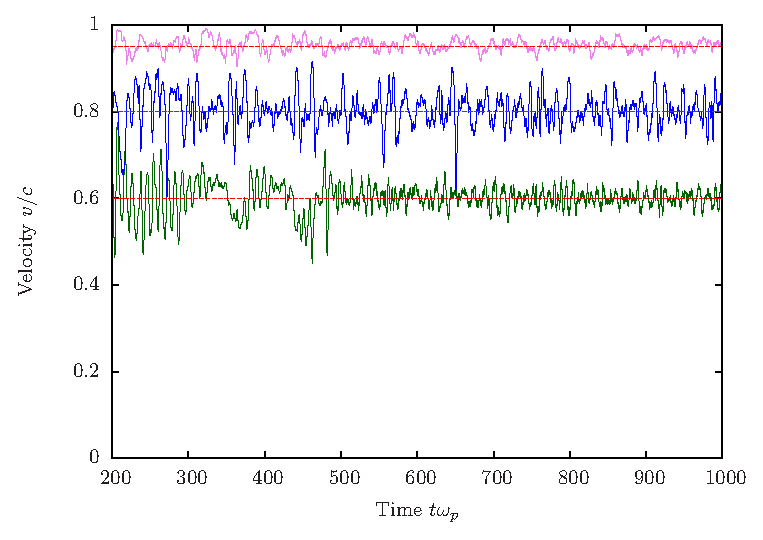
\includegraphics[width=0.8\textwidth]{pics/chap2/f4.eps}\\
%\plotone{f3b.eps}
    %\caption{(a) Evolution of the mean velocity of particles in the box, with $\alpha = 0.83$. The horizontal line plotted in red is $v=0.83$.
    % $x$-axis is in units of the plasma oscillation time $\tau = c/\omega_p$.
    %(b) The evolution of average momentum of particles in time, with $x$-axis in units of plasma oscillation time $\tau = c/\omega_p$.}
\caption[Evolution of $\bar{v}$ over time in the center of the domain]{Evolution
  of the hydrodynamical velocity $\bar{v}$ of the flow measured in the middle of
  the computational box. Three models are shown:
 % in a bin of size $4\lambda_p$ at , with
      $\alpha = 0.95$ (purple), $0.8$ (blue) and $0.6$ (dark green). In all
      three cases, the time-average value of $\bar{v}$ equals $\alpha$. }
    \label{fig:meanvelocity}
    \end{center}
\end{figure}
%%%%%%%%%%%%%%%%%%%%

%%%%%%%%%%%%%%%%%%%%
\begin{figure}% [h]
\begin{center}
% \epsscale{1}
%\epsscale{0.2}
% \plottwo{f5a.eps}{f5b.eps}
  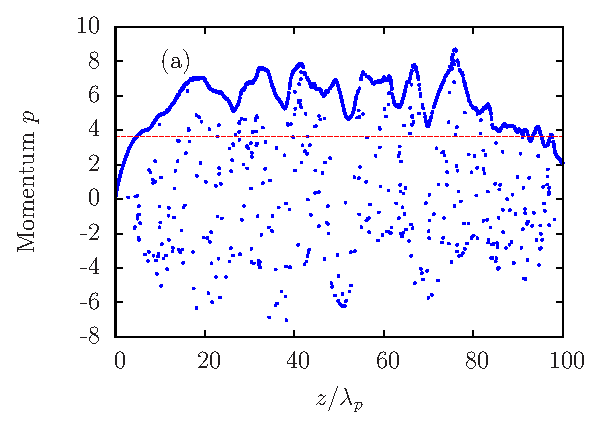
\includegraphics[width=0.6\textwidth]{pics/chap2/f5a.eps}\\
  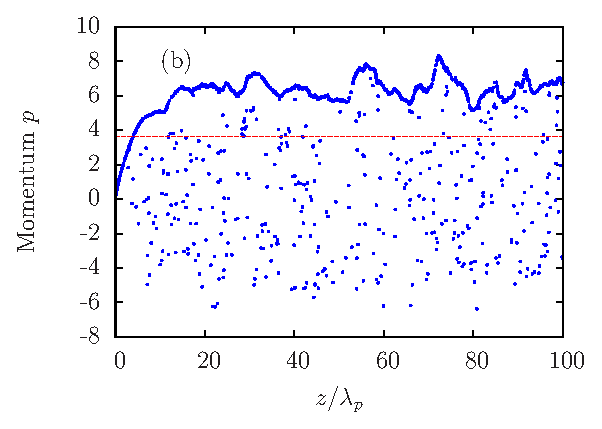
\includegraphics[width=0.6\textwidth]{pics/chap2/f5b.eps}
\caption[Snapshot of particle distribution]{Snapshot of 1000 randomly chosen particles in phase space for the flow
with $\alpha=0.8$ and $\bar{\beta}_0=0.2$.
%Purple curve shows the local mean (hydrodynamical) momentum $\bar{p}(z)$.
% inside a bin of size $\lambda_p/5$, and the r
Red dashed line shows the maximum momentum $p_{\max}$ for the steady cold solution
with the same $\alpha=0.8$ and $\beta_0=0.2$ (Section~3.1).
(a) Random snapshot for the simulation with box size $H = 100\lambda_p$.
(b) Another random snapshot of a similar simulation with a larger computational box
$H = 200\lambda_p$.
% Momentum is in units of $mc$.
}
\label{fig:phasetraj}
\end{center}
\end{figure}
%%%%%%%%%%%%%%%%%%%%


The moderate value of the hydrodynamic velocity does not, in principle, exclude
acceleration of a fraction of particles to much higher energies. We therefore also
studied the momentum distribution of particles in the flow.
Figure~\ref{fig:phasetraj}a shows a random snapshot of the particle distribution in the
phase space for the flow with $\alpha=0.8$.
We randomly chose 1000 particles between $z=0$ and $z=100\lambda_p$
and the figure shows their locations in the two-dimensional phase space $(z,p)$.
The simulation demonstrates the following:

(1) There is no high-energy tail in the momentum distribution.

(2) At each $z$, the momentum distribution has a pronounced narrow peak at
$p_{\rm peak}$. Thus, a large fraction of particles form a cold flow.
The momentum of cold particles
$p_{\rm peak}$ is slightly above the average (hydrodynamical) $\bar{p}(z)$, and
both are above (but comparable to) the value of $p_{\max}$ predicted by the
steady-state model.

(3) There is a low-energy wing in the momentum distribution which extends to
negative momenta (up to 10\% of all particles have $p<0$ in our sample model).
This broad component of the particle distribution has a
hydrodynamic velocity close to zero and does not contribute much to the
current density; however it makes a significant contribution to charge density.
In our sample model, about 20\% of particles reside in the broad component,
and this fact has a simple explanation. From the point of view of the cold stream
dynamics, the broad component provides a background that offsets the effect
of vacuum charge density $\rho_\mathrm{GJ}$ by the fraction of 20\%. This fraction
equals $1-\alpha$, so that the cold
stream may move with $v\approx c$ and carry $j_B$ without the mismatch in
charge density that would generate strong $E_\parallel$. In essence, the broad
component with backflowing particles allows the plasma to self-organize so that
the cold stream can keep $v\approx c$. This is in contrast to the steady-state
solution in \Sect~2, where all particles form a stream with a positive velocity
$v\neq\alpha$, which result in the periodic deceleration and acceleration of the
stream.

% This tail can be viewed as an effective background, which has a
% hydrodynamic velocity close to zero therefore does not contribute to the current
% density, but only changes the effective $\rho_\textrm{GJ}$. The system self-organizes
% such that the effective $\alpha$ becomes close to 1 after the initial acceleration layer.
% About 5-10\% of particles flow backward $(p<0)$.
%In our sample model, about 10 to 15\% of particles reside in the low-energy
%tail. This fraction is determined by the
%fact that the average velocity of the flow must equal $\alpha$ to conduct the required
%electric current. In our sample model $\alpha=0.8$ and hence less than 20\% of particles
%are allowed to have a small (or negative) velocity.
%About 5-6\% of particles flow backward ($p<0$).
%Note that the backflowing particles do not reach the surface $z=0$.
%This is prevented by the potential barrier of the accelerating layer with $\rho\gg\rho_\mathrm{GJ}$
%near the surface. All particles with $p<0$ are eventually accelerated to $p>0$ and
%escape the box through the outer boundary $z=H$.

(4) Both the fluid momentum $\bar{p}(z)$ and the peak momentum $p_{\rm peak}$
fluctuate in time (the corresponding curves in Figure~\ref{fig:phasetraj} move in time).
However, the qualitative form of the
phase-space distribution remains similar to that in Figure~\ref{fig:phasetraj}.

Note that the average momentum $\bar{p}$ does not correspond to
the average velocity $\bar{v}$ shown in Figure~\ref{fig:meanvelocity}, in the sense that
$\bar{p} \neq \bar{\beta}(1-\bar{\beta}^2)^{-1/2}$, because of the broad low-energy tail of
the distribution function. Compared with velocity average,
 the averaging of momentum gives a higher weight to particles with
 large $\beta$ because of the addition factor $\gamma$ in $p=\gamma\beta$.
The average velocity remains close to $\alpha c$, and the averaged momentum is
larger than $\bar{\beta}(1-\bar{\beta}^2)^{-1/2}$.

It should also be noted that the pronounced narrow stream and the broad low-energy stream together
form a two-stream system. Conventionally one would expect the configuration to suffer
from standard micro-instabilities. However, we do not observe such kind of instabilities here.
One important reason is that the
flow remains turbulent even after establishing this quasi-steady state. The momentum
of particles in the colder stream oscillates both in time and space, thus any particle
would not be able to interact with a single wave for extended period of time. In this
case, exponential growth of particular waves cannot occur, which kills the instability.

As seen in Figure~\ref{fig:phasetraj}a, the flow momentum $p_{\rm peak}$ decreases
near the outer boundary of the computational box $z=H$.
This is an artifact of the boundary condition (free escape with no backflow), which
suppresses backflow density near the boundary. As a result, a modest negative electric
field is induced near the boundary, decreasing $p_{\rm peak}$ so that the flow carries
the required electric current $j_B$.
For comparison, Figure~\ref{fig:phasetraj}b shows a random snapshot of a similar model (in the same interval $0<z<100\lambda_p$) that has twice as large computational box, $H=200\lambda_p$.
As we increase $H$, the boundary effect moves away to larger $z$, affecting the flow
properties only at $z\approx H$. The fraction of backflowing particles measured inside the
box remained unchanged at $\sim$10\%.

%%%%%%%%%%%%%%%%%%%%
\begin{figure}[h]
\begin{center}
%\epsscale{0.25}
   % \epsscale{1.0}
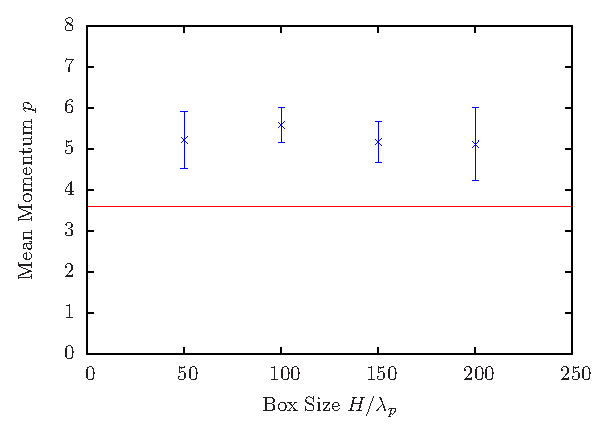
\includegraphics[width=0.7\textwidth]{pics/chap2/f6.eps}
\caption[Mean and standard deviation of particle momentum at the center of the
simulation box]{Mean expectation and standard
  deviation for the fluctuating hydrodynamical momentum of the flow measured at
  the center of the computational box. Four simulations are shown, with box
  sizes $H/\lambda_p=50$, 100, 150, and 200; all four simulations have the same
  parameter $\alpha=0.8$. Red line shows the maximum momentum predicted by the
  steady state model with $\alpha=0.8$.}
% Comparison of the mean momentum in a bin of size $2\lambda_p$ at the center of the box over one light-crossing time of $H_1=100\lambda_p$, plotted for different numerical parameter $H/\lambda_p$, with the same $\alpha = 0.8$. Error bar indicates the standard deviation of the mean momentum.}
\label{fig:zetacompare}
\end{center}
\end{figure}
%%%%%%%%%%%%%%%%%%%%

We also checked whether the flow momentum depends on the size of the computational
box. We ran several simulations with the same $\alpha = 0.8$ and different box sizes
$H$. In each simulation, we measured the fluid momentum $\bar{p}$ in the center of
the box (using a bin $\Delta z=2\lambda_p$) at time $t=100\omega_p^{-1}$.
The results are shown in Figure \ref{fig:zetacompare}.
There is no systematic variation in $\bar{p}$ with the box size; the small variations
($\lesssim 10$\%) are consistent with the fluctuations of $\bar{p}$ in time for each model.

The other numerical parameter of the simulations is $N_p$ (\Sect~3). We checked
that  the results do not depend on $N_p$ as long as it is large; variations in $N_p$
around $\sim 10^4$ did not change the measured parameters of the flow.


%#################################################################

\section{Mixed ion flow and two stream instability}
\label{sec:pc-ions}


If $j_B>0$ (which is equivalent to $\rho_\mathrm{GJ}>0$ for $\alpha>0$), the
charge-separated flow puled out from the polar cap is made of ions.
Different species of ions may end up in such a flow, and they will be
accelerated to different velocities.

The mixed ion flow shares many features with the identical-particle model
studied in the previous sections. Steady state solutions exist for such flows,
which can be obtained using the method described in \Sect~\ref{sec:solutions}.
Ions with different masses and charges move with different hydrodynamical
momenta and co-exist in a common, periodic electrostatic potential.
This steady solution
is prone to kinetic instability similar to that described in Sections~2 and 4.
%
There is, however, an important new feature: the ion streams with
different hydrodynamical momenta are prone to two-stream instability.

% We modified our numerical setup to investigate the later possibility.
To study the behavior of the mixed ion flow we use a simplest modification of
our numerical simulation. Consider a mixture of protons and helium nuclei
(alpha-particles).
The particle injection at $z=0$ now consists of two ions species; they have
charges $e_1$ and $e_2=2e_1$, and masses $m_1$ and $m_2=4m_1$.
The two species are injected with equal rates $\dot{N}_1=\dot{N}_2$.
% and with equal velocities $v_0=0.4c$.
Then alpha-particles carry electric current $j_2=e_2\dot{N}_2$ that is
two times larger than the proton current $j_1=e_1\dot{N}_1$. Thus,
$j_2=(2/3)j_B$ and $j_1=(1/3)j_B$ are maintained at the boundary.

To define a charateristic plasma skin depth $\lambda_p$ we use
equation~(\ref{eq:lambda}) where we replace $e,m,j_B$ by $(e_1,m_1,j_1)$
or, equivalently, by $(e_2,m_2,j_2)$ (note that $e_2j_2/m_2=e_1j_1/m_1$).
The characteristic plasma frequency is defined by $\omega_p=c/\lambda_p$.

% proton and helium respectively.
%They are injected with the same number density???????
%Their injection rates are equal???????
%  and uniform momentum (cold injection), and
% $j_B$ is maintained at the boundary.
% The rest of the simulation setup is similar to that described in section \ref{sec:setup}.

% In fact, a steady state solution exists for such a configuration, and can be found
% using similar method as described in section \ref{sec:solutions}. The solution of
% the electric potential can be found by numerical integration. It again has a periodic
% structure, and the two streams flow independently in the background potential.
% However, this solution is prone to the
% same kinetic instability as the identical particle stream. In addition to that, we
% also observed the development of two-stream instability which further mixes the
% particles in momentum space.

%%%%%%%%%%%%%%%%%%%%%%%%%%%%%%
\begin{figure}[h]
%\epsscale{0.25}
  % \epsscale{1.0}
\begin{center}
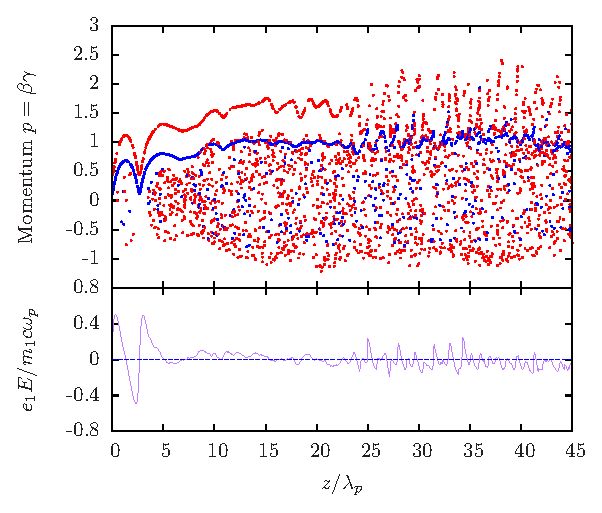
\includegraphics[width=0.8\textwidth]{pics/chap2/f7.eps}
\caption[Snapshot of mixed ion flow]{Snapshot of the mixed ion flow with
  $\alpha=0.4$ at time $t = 10^3\omega^{-1}_p$. Top panel shows the phase space
  distribution, where red dots represent protons and blue dots represent helium
  ions. Bottom panel shows the electric field. }
\label{fig:2stream}
\end{center}
\end{figure}
%%%%%%%%%%%%%%%%%%%%%%%%%%%%%%

Figure~\ref{fig:2stream} shows a snapshot of the phase-space distribution of
ions long after the beginning of the simulation. In this sample model
$\alpha=0.4$; the modest value of $\alpha$ (not close to unity) implies modest
Lorentz factors of particles and fast development of instabilities.
%
% The result of the simulation can be summarized quite well by figure \ref{fig:2stream}.
% The figure illustrates the following features:
The flow exhibits the following features:
% \medskip

\noindent
(1) One period of the steady state solution is reproduced near the injection
boundary $z=0$. The period $z_0\approx 3\lambda_p$ agrees with the result
from numerical integration of the corresponding steady state model.
(This feature is stable in our sample model
because we chose a relatively large injection velocity $v_0=0.4c$.)
% \medskip

\noindent
(2) At larger $z$ the periodic flow becomes unstable and develops into a
configuration similar to that in Figure~5, except that now we have {\it two}
cold variable streams. Besides the cold streams, there is a broad distribution
of ions with smaller momenta and a negligible hydrodynamic velocity.
% which forms an extended wing of the
% distribution function at low momenta.
In our sample model $\alpha=0.4$ and
correspondingly the broad component is self-organized to contain up to
$\sim 60\%$ of particles, so that the streams may move with a relativistic speed
without mismatch in charge density that would generate strong electric fields.
% in both streams of the flow,
% As discussed in \Sect~4, the effect of the broad component on the stream
% dynamics may be viewed as a background that reduces the effective
% $\rho_\mathrm{GJ}$ by a factor of 0.4.
% making the effective $\alpha$ close to unity.
% \medskip

\noindent
(3) Further from the boundary (at $z>20\lambda_p$), the two streams
develop a two-stream instability. The growth rate of the instability may be
estimated using an idealized model of two streams with densities $n_1$,
$n_2$ and velocities $v_1,v_2$. It is straightforward to derive the dispersion
relation for Langmuir modes with frequency $\omega$ and wave-vector $k$
% (e.g. Melrose 1986);
\citep[e.g.][]{melrose_instabilities_1986};
it gives,
\begin{equation}
\label{eq:disp}
    1-\frac{\omega_1^{2}}{\gamma_1^3(\omega - kv_1)^2} - \frac{\omega_2^{2}}{\gamma_2^3(\omega - kv_2)^2} = 0,
\end{equation}
where $\omega_1^2=4\pi n_1 e_1^2/m_1$ and $\omega_2^2=4\pi n_2 e_2^2/m_2$.
Using $\omega_1\approx\omega_2\approx\omega_p$ and the characteristic values
of velocities $v_1,v_2$ from our simulation, we find from equation~(\ref{eq:disp}) that
the most unstable modes have $\omega$ comparable to $\omega_p$ and their
growth rate is $\Gamma\sim 0.1\omega_p$.
% The instability does not happen
% at smaller $z$ because it takes some time to grow. We can estimate the
% growth rate by solving equation (\ref{eqn:twostream}) numerically. For
% modes with reasonable wavelength the growth rate is on the order of
% $\Gamma \sim 0.1\omega_p$.
The distance over which Langmuir waves are amplified is roughly
 $10\lambda_p$.
% to develop siginificant instability, which agrees with our simulation.
As a result of the instabiility, the two streams are smeared out at large $z$,
in particular the stream of lighter ions.
No significant particle acceleration is seen in the simulation.

% The standard dispersion relation for longitudinal Langmuir waves in a two-stream
% configuration is given by (see e.g. Boyd and Sanderson, \emph{The Physics of Plasmas})
% where subscripts 1 and 2 refer to the two ion streams; $\omega_1$ and
% $\omega_2$ are their plasma frequencies. The frequency
% of the fastest growing modes is $\omega\approx 2\gamma_1^{1/2}\omega_1$,
% and the growth rate of the instability is $\Gamma\sim 0.1\omega_p$.


%#############################################################

\section{Discussion}
\label{sec:pc-discussion}

We have presented detailed one-dimensional time-dependent simulations
of the plasma flow extracted from the polar caps of neutron stars.
The simulations provide a fully kinetic description of the flow,
with self-consistent electric field and particle distribution function.
In this chapter, we focused on the regime $0<\alpha<1$, where $\alpha$ is the main
parameter of the flow defined by equation \eqref{eq:alpha}.
In agreement with the estimates of B08, we find that
the particles are accelerated to Lorentz factors,
\begin{equation}
\label{eq:gam2}
   \gamma\approx \frac{1+\alpha^2}{1-\alpha^2},
 \end{equation}
and are not capable of igniting pair creation.
In this sense, flows with $0<\alpha<1$ are ``dead.''
They are sustained by a modest voltage, oscillating in space and time.

The simulations show how a kinetic instability develops and disrupts the ideal
periodic structure found in analytical models of the dead zone (\Sect~2).
We find that the momentum distribution function has two distinct parts --- a
variable ``cold stream'' and a broad wing at low momenta, which includes particles
flowing backward to the polar cap. Even though the flow is turbulent, it shows
no signs of particle acceleration to energies higher than that of the cold stream.

%-----------------------
% Note that the analysis is LOCAL, i.e. the behavior of the flow is controlled
% by the local value of $\alpha=j_B/c\rho_\mathrm{GJ}$, as long as the flow is charge
% separated, and applies to any magnetospheres
% (not necessarily dipole). It also extends to the case where  in a relativistic
% backflow of opposite charge is present; the density of this backflow can be
% included by changing the effective $\rho_\mathrm{GJ}$.
%-----------------------
%MELROSE

The value of parameter $\alpha$ depends
on the location and geometry of the polar cap.
A simplest magnetospheric configuration is that of a centered dipole. Then
the parameter $\alpha$ depends on the angle between the magnetic and spin axes,
$\xi$; besides, it varies across the polar cap. For nearly
aligned rotators ($\xi\approx 0$),
$0<\alpha<1$ in the central part of the polar cap and $\alpha<0$
in a ring-shaped zone near the edge of the polar cap
% (Timokhin 2006; Parfrey et al. 2012).
\citep{timokhin_force-free_2006,parfrey_introducing_2012}
In this case, the dead zone occupies the
central part of the polar cap, and $e^\pm$ discharge must be confined to the ring,
% only the ring is expected to produce $e^\pm$ discharge,
% and radio emission.
matching the phenomenological ``hollow cone'' model of pulsar emission.
% suggested by Goldreich \& Julian (1969).
%  \cite{1969ApL.....3..225R}.
In contrast, the polar cap of an orthogonal rotator ($\xi\approx \pi/2$) has
$|\alpha|\gg 1$, which
% corresponds to efficient particle acceleration and
enables $e^\pm$ discharge
% and radio emission from
for the entire polar cap.
At arbitrary misalignment $0<\xi<\pi/2$,
the values of $\alpha$
% for various $\xi$ is
can be provided by global three-dimensional simulations
of the magnetospheric structure
% (e.g. Spitkovsky 2006)
\citep[e.g.][]{spitkovsky_time-dependent_2006}
and should play a key
role for the geometry of the radio beam.


% On the other hand, in models where $\alpha$ changes across the polar cap, this result provides a description of the ``dead'' regions of the polar cap. Specifically in \cite{1969ApL.....3..225R} it was found that for some pulsar polar caps $\alpha$ changes sign near the boundary, thus creating a ring structure on the polar cap. Inside the ring we have $0<\alpha<1$ which is the ``dead'' region whereas outside the ring we have $\alpha<0$ which will create hugh particle acceleration. If this result can be extrapolated to pulsars which are slightly unaligned, it would predict radio emission patterns with a cone structure, where plasma activity and emissions only take place on magnetic field lines originating near the edge of the polar cap, and the region in the center produces no emission.  Further investigation of this relation would be very interesting.

% This simulation does not include pair creation near the polar cap. Our next goal is to modify the numerical code to include pair creation and investigate the time dependence of the polar cap thickness, for parameters of $\alpha > 1$ or $\alpha < 0$.

We presented our results using plasma skin depth $\lambda_p$ as a unit of
length and particle rest-mass $mc^2$ as a unit of energy. In this form, the results
do not depend on the charge or mass of the particles extracted from the polar cap,
as long as our assumption --- that the flow is made of identical particles --- is
satisfied. In particular, equation~(\ref{eq:gam2}) is valid for both electron flow
($\rho_\mathrm{GJ}<0$) and ion flow ($\rho_\mathrm{GJ}>0$), and the phase-space
distribution shown in Figure~5 describes both cases.
Note that the accelerating voltage is proportional to the particle mass;
voltage implied by equation~(\ref{eq:gam2}) is different for ions and electrons by
the factor of $m_i/m_e\sim 2\times 10^3$.
The relatively high voltage in the ion flow,
$e\Phi\approx\gamma m_ic^2 (1+\alpha^2)/(1-\alpha^2)$,
is still hardly sufficient to ignite $e^\pm$ pair discharge by a seed electron or positron.

The identical-particle model may not hold for an ion flow; in this case,
new effects may enter the problem.
Firstly, heavy ions pulled out from the polar cap may not be completely ionized
and begin to lose electrons as they are accelerated and interact with the X-rays
above the stellar surface; this process effectively creates new charges,
reminiscent of pair creation
% (e.g. Jones 2012).
\citep[e.g.][]{jones_post-glitch_2002}
Secondly, the ion flow may be a
mixture of different nuclei which will be accelerated to different Lorentz factors.
The mixed ion flow is prone to two-stream instability, possibly leading to formation
plasma clumps and generation of coherent radio emission.
In our simulations, we observe the expected two-stream instability,
however do not observe significant structure (clumps) in the turbulent flow.
This may change in three-dimensional simulations.
The frequency of excited waves $\omega\approx 2\gamma_1^{1/2}\omega_1$
is in the radio band, and coherent emission from clumps could create bright
coherent emission. It remains to be seen whether this mechanism
can contribute to the pulsar emission. If it does,
it would create an additional component of the radio pulse.
In the case of aligned rotator, the additional component would be generated in
the central region of the polar cap, leading to a ``hollow cone + core'' structure of
the radio pulse.

% In the case of an ion flow,
% It was proposed that
The charge-separated model of the dead zone can be modified to include possible
backflowing particles from distant parts of the open field-line bundle
(e.g. from a pair-producing outer gap). These particles can contribute to the current
density and also serve as an
additional background charge density, which may be modeled as a contribution to the
effective ``vacuum'' charge density  $-\rho_\mathrm{GJ}$.
This would change the effective $\alpha$
% (Lyubarsky 1992; B08),
\citep[][B08]{lyubarskij_current_1992},
most likely reducing it.
% In particular, if an outer gap produces relativistic $e^\pm$ pairs and sends part of them
% toward the star.

An outer gap is expected to form in a charge-separated flow near the null surface
$\mathbf{B}\cdot\bOm=0$
% (Cheng \& Ruderman 1986)
\citep{cheng_energetic_1986}
. On a given field line, the outer gap will be screened if it is loaded by multiple $e^\pm$ pairs
produced by discharge at the polar cap.
% near the star and loads the field lines with $e^\pm$ flow of a high multiplicity.
Thus, suppression of $e^\pm$ discharge near the field line footpoint is
an essential condition for the existence of an outer-gap accelerator.
% This condition is satisfied only in the dead zone.
Therefore, one can expect an outer gap to form on
field lines with footpoints in the dead zone.

% Outer gap; Parfrey et al. (2012)

We did not simulate in this chapter flows with $\alpha>1$ or $\alpha<0$;
in these cases particles must be strongly accelerated.
This regime leads to an $e^\pm$ discharge that must be unsteady,
with a significant intermittent backflow (B08).
A model for oscillating discharge can be studied in hydrodynamical approximation
\citep{levinson_large-amplitude_2005}
, however a fully kinetic description is essential.
We defer the kinetic time-dependent simulations with pair creation
to a future paper.


% Local Variables:
% TeX-master: "../thesis"
% zotero-collection: #("16" 0 2 (name "Thesis"))
% End:
